% Chapter Template

\chapter{Implementation} % Main chapter title

\label{implementation} % Change X to a consecutive number; for referencing this chapter elsewhere, use \ref{ChapterX}

\lhead{Chapter 5. \emph{Implementation}} % Change X to a consecutive number; this is for the header on each page - perhaps a shortened title

%----------------------------------------------------------------------------------------
%	SECTION 1
%----------------------------------------------------------------------------------------

Sed ullamcorper quam eu nisl interdum at interdum enim egestas. Aliquam placerat justo sed lectus lobortis ut porta nisl porttitor. Vestibulum mi dolor, lacinia molestie gravida at, tempus vitae ligula. Donec eget quam sapien, in viverra eros. Donec pellentesque justo a massa fringilla non vestibulum metus vestibulum. Vestibulum in orci quis felis tempor lacinia. Vivamus ornare ultrices facilisis. Ut hendrerit volutpat vulputate. Morbi condimentum venenatis augue, id porta ipsum vulputate in. Curabitur luctus tempus justo. Vestibulum risus lectus, adipiscing nec condimentum quis, condimentum nec nisl. Aliquam dictum sagittis velit sed iaculis. Morbi tristique augue sit amet nulla pulvinar id facilisis ligula mollis. Nam elit libero, tincidunt ut aliquam at, molestie in quam. Aenean rhoncus vehicula hendrerit.

\section{Case 1: Gas dispersion in a simplified urban area}
%The problem investigated in this work is gas dispersion of neutral gas in a velocity field through four cubic blocks.
%Similar simulations have been done in CDP and Fluent which are compared to data from a wind-tunnel experiment performed by ALAN.

The scenario investigated in this work is dispersion of a neutral gas in a rectangular tunnel
with four cubic blocks placed as obstacles. The blocks have sides $h = 0.109$m and represent a 
set of buildings forming a street canyon. The gas is released from a circular source on 
ground level and
is translated by the wind field through the canyon, see figure~\ref{fig:layout}.
In this figure $h$ have been used as the length scale. The dotted lines
indicates the positions where data is collected.
%
\begin{figure}[h]
	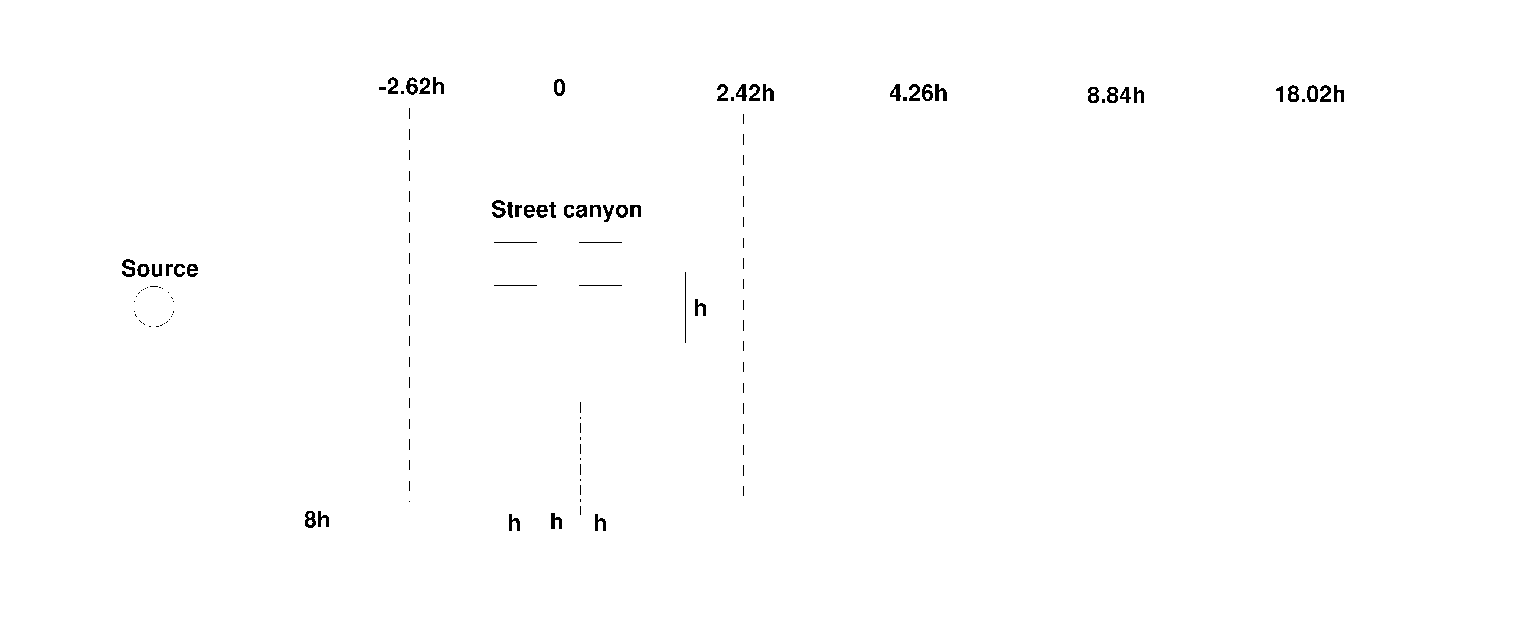
\includegraphics[width=1.1\textwidth]{Figures/layout.eps}
	\caption{Schematic overview of the domain from above. The data is collected along the dotted lines.}
	\label{fig:layout}
\end{figure}
%

Scaling the domain with the size of the boundary layer $H =1$m restricts it to
the box $0.0\leq x/H \leq 4.96,-1.75\leq y/H \leq 1.75, 0\leq z/H \leq 1.5$.
The four cubic boxes are centered around $(1.4315,0)$ with a distance $h$ between each box.
The source is placed with its center in $(0.396,0)$ and radius $r = 0.0515$.
The grid used for the computations consists of 4425 elements and with a polynomial degree of
12 the total number of nodes $N\approx 7,6$mill. 

The simulations are performed using Large Eddy Simulation (LES) 
with the dynamic Smagorinsky-Lilly subgrid-scale model. 
The release of gas will result in a plume that is advected with the wind field. The size and 
shape of the plume at the indicated positions in figure~\ref{fig:layout} are compared with 
experimental data and simulations performed in Fluent and CDP\@. 
The wind-field in the tunnel is created by an inflow condition that is defined from previous 
simulations in CDP~\cite{eriksson}.
For clarification some of the variables repeteadly mentioned throughout this thesis will be 
stated explicitly in table~\ref{tab:variables}.
\begin{table}
    \centering
    \begin{tabular}{c c c c}
        Variable & value & unit & commentary \\ \hline
        $H$   & $1$ & m & length scale of the domain \\ 
        $h$   & $0.109$ & m & the sides of the cubic boxes\\ 
        $Q$   & $50$ & dm$^3$/min & gas release from source \\ 
        $U_{ref} $*& $\approx1.08$ & m/s & reference value of $U$ \\
    \end{tabular}
    \caption{Essential variables, *this value is calculated as a time average of the velocity in 
        x-direction at a point far away from the floor and walls and will therefore 
        vary a small amount from case to case. }
    \label{tab:variables}
\end{table}


\section{Case 2: Drag and lift on a cylinder}
A standard benchmark case for flow solvers is presented in ~\cite{benchmark}.
The case is to calculate the drag and lift coefficients on a cylinder in a rectangular channel.
The setup for the domain and boundary conditions are given in figure~\ref{fig:cylinder}.
The constants applied in the description of the geometry and the coefficient scales are listed 
in table ~\ref{tab:case2consts}.
%
\begin{table}[h]
    \centering
    \begin{tabular}{c l l}
     Constant & Value & Property \\ \hline
    $H$ & $0.41\text{m}$ & Width and height for the channel \\
    $D$ & $0.1\text{m}$ & Diameter of the cylinder and length scale \\
    $U$ & $0.2\text{m/s}$ & Velocity scale \\
    $\nu$ &  $ 10^{-3}\text{m$^2$/s}$ & Kinematic viscosity of the fluid \\
    $Re$ & $20$ & Reynolds number \\ 
    \end{tabular}
    \caption{Constants for case 2}
    \label{tab:case2consts}
\end{table}
%
The flow is laminar with Reynoldsnumber $Re=20$ so all the 
challenges arising when dealing with turbulent flow does not come to play in this case. 
The case will yield a steady state solution at which point the coefficients are calculated
and compared with the reference solutions.
\begin{figure}[h]
    \centering
    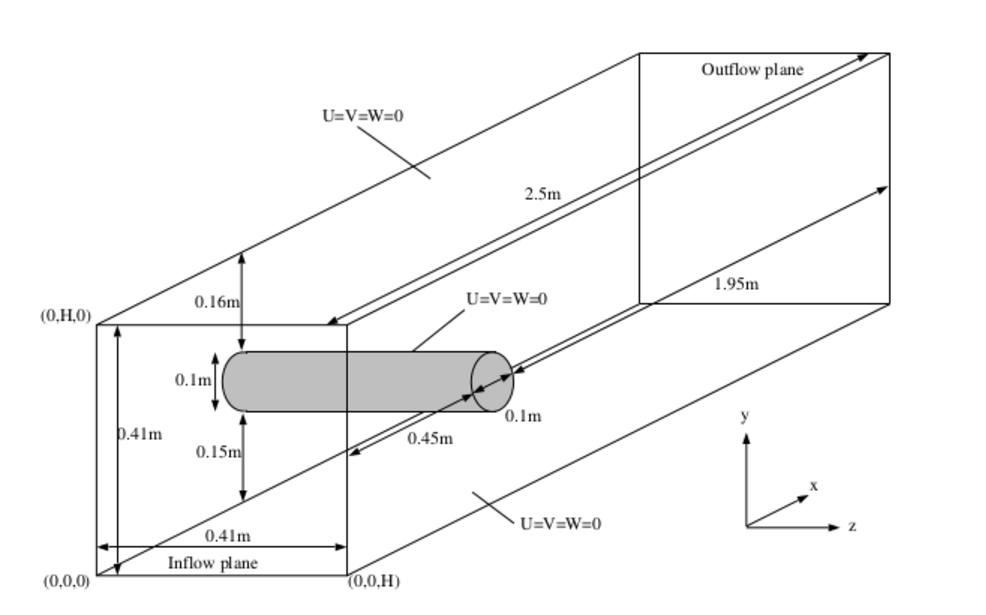
\includegraphics[width = 1.0\textwidth]{Figures/cylinder.pdf}
    \caption{Computational domain and boundary conditions.}
    \label{fig:cylinder}
\end{figure}
The spectral element method applied in Nek is known to be an accurate
solution method and is expected to 
provide a very good result in a test-case like this.
The drag and lift forces on an surface $S$ are given as 

\begin{align}
    F_D = \int_{S}(\rho \nu \frac{\partial v_t}{\partial n}n_y-pn_x)dS 
    \qquad , \qquad
    F_L = -\int_{S}(\rho \nu \frac{\partial v_t}{\partial n}n_x+pn_y)dS.
    \label{eq:dragnlift}
\end{align}

The coefficients corresponding to these forces known as the drag and lift coefficients 
are given by the formulas 
\begin{align}
    c_D = \frac{2F_D}{\rho U^2 D H}
    \qquad , \qquad
    c_L = \frac{2F_L}{\rho U^2 D H}.
    \label{eq:dragnliftcoeffs}
\end{align}
Nek provides functions for calcuting lift and drag on any user-specified object.
The function is called \verb|drag_calc(scale)|, with the input parameter 
defined by the user, for this case \verb|scale|$=2/(\rho U^2DH)$.  
Apart from this a \verb|set_obj()| has to be modified in order to create an object 
which consists of all the faces on the cylinder.
Let $x,y$ be points in the computational domain, $x_c,y_c$ be the coordinates to the 
center line in the cylinder and $0<tol\ll1$ be some user defined tolerance. The faces that belong to the cylinder can then be found by 
looping over all elements and their faces evaluating $\epsilon = \sqrt{(x-x_c)^2+(y-y_c)}$.
If $\epsilon < tol$ for an entire face then this face is known to 
belong to the cylinder and is added to the object. Nek also allows the user to specify multiple objects 
assigning the faces of interest to object 1, object 2 etc. The geometry and mesh 
for this case was generated in ICEM, and the total number of elements are 2070. 
For the final calculation polynomial degree $P = 11$ was applied leading to a 
total of $N = 2755170$.

%
\begin{figure}[h]
    \centering
    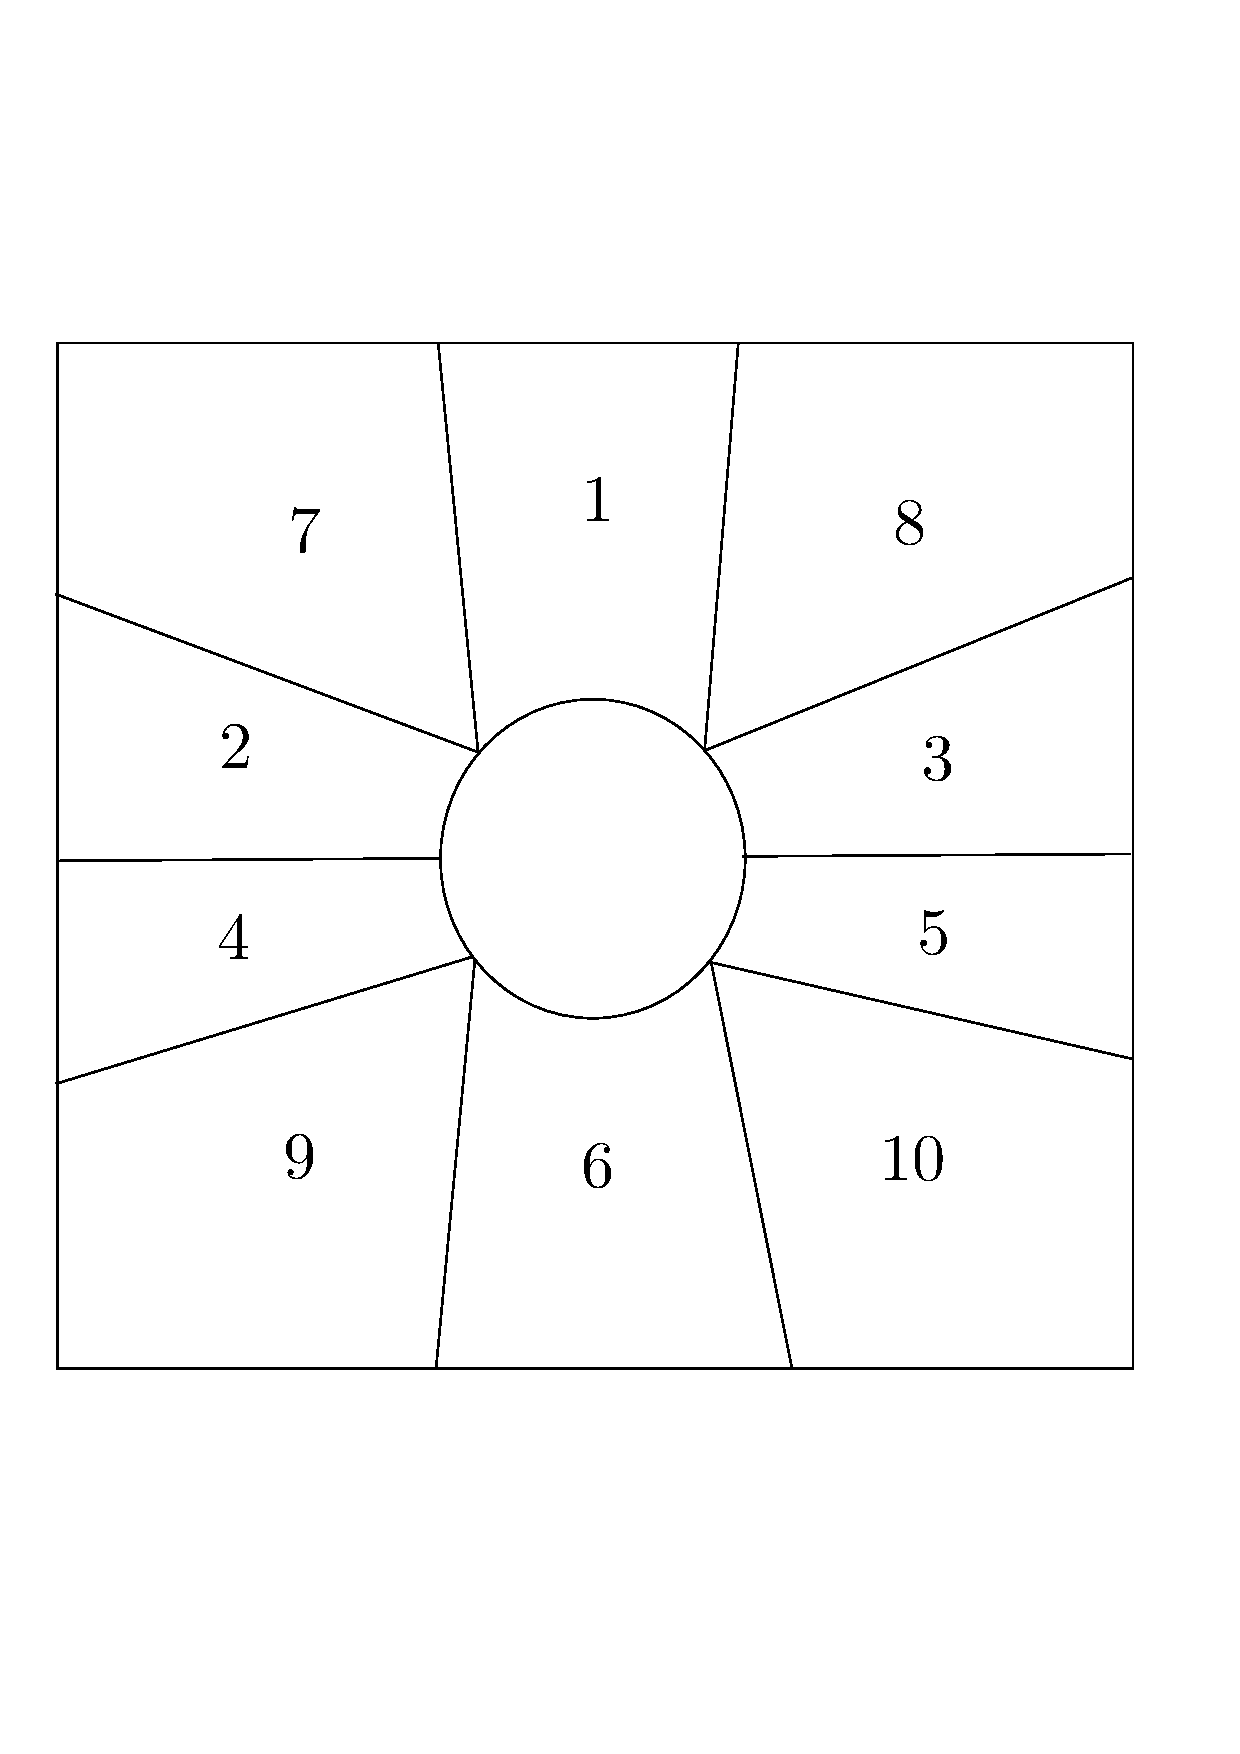
\includegraphics[width = 0.4\textwidth]{Figures/cyl_elem.pdf}
    \caption{Initial mesh around cylinder.}
    \label{fig:cyl_elem}
\end{figure}
%
Initially this case was solved using a second degree polynomial to describe the circle segments
corresponding to each element. The mesh around the cylinder is illustrated in figure~\ref{fig:cyl_elem}.
Note that these elements was split in three, in order to obtain 
a finer mesh in the region of interest. Of the elements numbered in~\ref{fig:cyl_elem}
only the first six contains edges on the cylinder.Hence the second order polynomials 
describing the curved edges describe approximately $\Theta = 360^{\circ}/(6\cdot 3) = 20^{\circ}$
of the complete circle. There is no computational reason 
for not incorporating an order $n=P$ approximation of the circle segments eliminating 
this approximation error. An algorithm was therefore implemented as an extension to the
currently available features regarding curvature on edges.
The full description of the algorithm is presented in 
chapter~\ref{xyzarc}. The importance of the error resulting from the second degree approximation
of the circle segments are presented in chapter~\ref{results}.
%
%
%
\section{Advances in the mesh-generation routine} \label{xyzarc}
The routine xyzarc:

The gordon hall algorithm was already implemented as a function in Nek, with the gll-points,plynomial degree and some initial 
coordinates to the element. The algorithm creates a distribution of the internal gll-points in each element. 
If the element consists of linear edges the only necessary input are the vertices, but by specifying the points on edges and faces
the algorithm creates a logical distribution of the internal GLL-points to a deformed element. 

The curved edge is specified in the .rea file and the routine genxyz() processes the input of each edge. 
By specifying the radius and the circle center genxyz calls the routine xyzarc() which performs the following algorithm;

    $a,b$ will be the two endnodes of the edge 
    $c$ will be the midnode, $s$ will be the arc length, $\theta$ will be the full angle of the circle sector, $cc$ is the center coordinates.
    $g$ will be the vector containing the GLL-points in $[-1,1]$. $r$ will be the radius.

	%/* Pseudo code */
%define interpolation algorithm 
%\textbf{\textbf{for}} each timestep \emph{T}
  %Read inflow
  %\textbf{for} each node \emph{N} and velocity component \emph{V} on inflow boundary 
    %\emph{V}(\emph{N}) = doInterpolation(N)
  %\textbf{endfor}
  %solve
%\textbf{endfor}
\begingroup
\fontsize{12pt}{14pt}
\begin{lstlisting}[escapechar=|]
 l = a-b                       # vector between the corner nodes
 c = (a+b)/2                   # midpoint location
 h = c-cc                      # height of the framed triangle
 |$\theta$| = arctan(abs(l)/2abs(h))    # half the angle of the circle sector
 s = r*|$\theta$|                       # arclength
 g' = g*|$\theta$|                      # angles to the gll-points on the circle-sector
 #---------- Finding the intersecting points ----------#
 #---- x on the line l, and extend x-cc to the arc ----#
 |\textbf{for}| k in range(lx1):          # For the number of nodes in one direction
    |$\alpha$| = h*tan(g'[k])           # Offset from the midpoint on l
    x = c-|$\alpha$|*l/abs(l)           # Actual coordinate on l
    m = x-cc                   # hypothenus of the imposed triangle
    edge(k) = cc+r*m/abs(m)    # final coordinate on the arc
\end{lstlisting}
\endgroup
These lines creates the wanted egde curved as a circle sector corresponding to the radius and circle center given.
The remaining operation is to call the gordon hall algorithm and create the internal GLL-points defined by the edges 
provided. The figure~\ref{fig:curvature} illustrates the geometry on which the algorithm is performed.
Notice that the algorithm assumes that the center is somewhere on the plane defined as all the 
points with equal distance to both $a$ and $b$.


\begin{figure}[h]
    \centering
    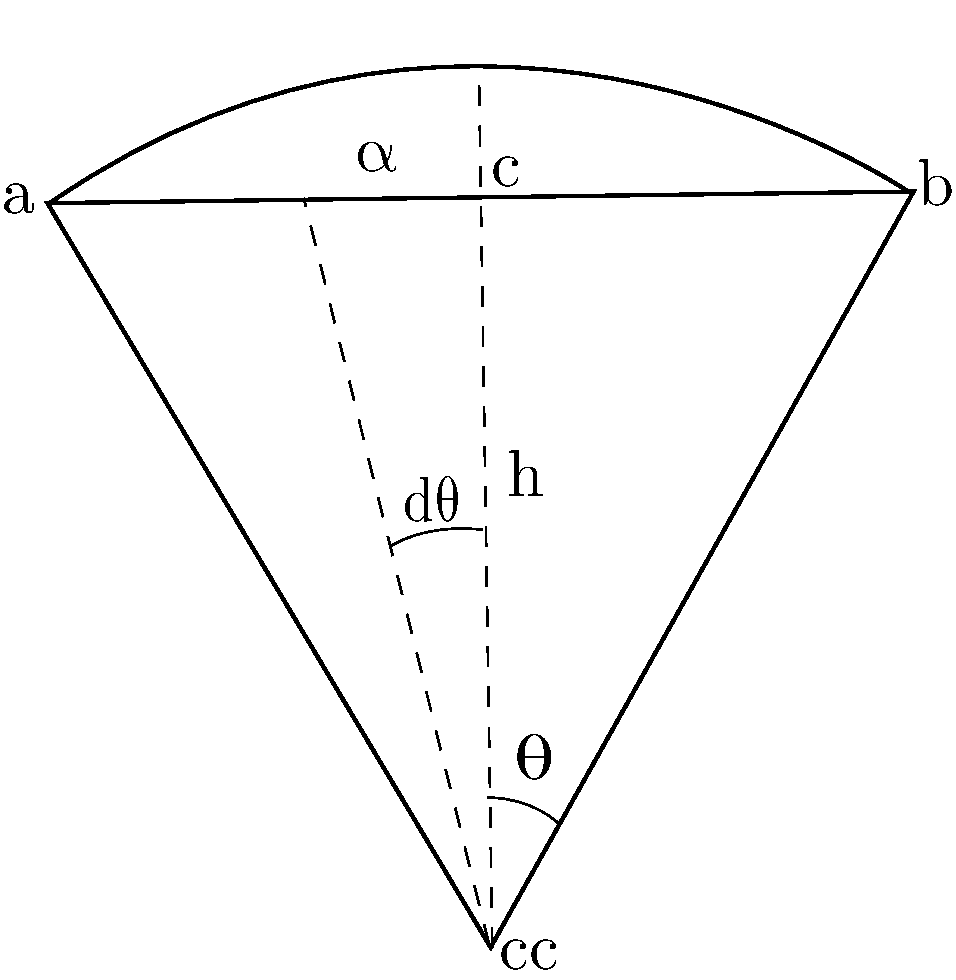
\includegraphics[width = 0.5\textwidth]{Figures/curvature.pdf}
    \caption{A sketch of the curved edge and the variables necessary to calculate the projection}
    \label{fig:curvature}
\end{figure}


\begin{itemize}
	\item initial script
	\item changes and modifications
	\item performance testing
	\item pitfalls
\end{itemize}


